\documentclass[a4paper,10pt]{scrartcl}

% Deutsche Umlaute (Mac)
\usepackage[applemac]{inputenc}

% Deutsche Umlaute (Windows)
%\usepackage[ansinew]{inputenc}

% Einbinden von Bildern
\usepackage{graphicx}
\usepackage{todonotes}

% SeitenflŠche etwas mehr ausnutzen
\usepackage{geometry}
\geometry{a4paper,left=30mm,right=30mm, top=1cm, bottom=3cm}

% Kein EinrŸcken bei zweispaltigen Bildunterschriften
\usepackage[normal]{caption}

% == Lottes Änderungen ===
% großer erster Buchstabe
\usepackage{lettrine}
\usepackage{graphicx}
\usepackage{caption}
\usepackage{subcaption}

% Glossary benutzen
\usepackage{glossaries}
\loadglsentries[main]{glossary}
\makeglossaries

% zeilenumbrüche in tabellen
\newcommand{\specialcell}[2][c]{%
  \begin{tabular}[#1]{@{}c@{}}#2\end{tabular}}

\begin{document}

% Titel
\title{Hybrid routing for the Internet of Things}
\subtitle{challenges and opportunities}
\author{Lotte Steenbrink}
\date{Wintersemester 2014/15}
\maketitle

\begin{abstract}
I am an abstract. Write me!
\end{abstract}

\section{Introduction}
\label{sec:Intro}
%==============================================================================
The rest of this paper is organized as follows. \todo{TODO! (where do I put this?)}
The goal of this paper is thus to explore how hybrid routing can be advanced with the \gls{IoT} in mind, building on the foundation which research on \gls{MANET} routing of the past 15 years has built.\todo{find a place for this}\\ 

\subsection{What is the Internet of Things?}
\label{subsec:IoT}
%==============================================================================
The \gls{IoT} envisions autonomous communication between tiny computers installed in everyday objects such as furniture, toys, clothing, or tools with the goal of making them smarter and improving their user experience. IoT devices typically are very constrained devices with no constant power supply. Therefor, they need to be resourceful in terms of computation, storage, RAM and energy usage.
To communicate amongst each other, IoT nodes form spontaneous, wireless mesh networks.
The vision of the Internet of Things is rapidly becoming reality, and with its rise, new demands for routig protocols that serve these kinds of mesh networks surface which cannot be optimally served by either reactive or proactive routing protocols alone.\\
One example for this may be the lighting system in a smart home: Each lamp needs to maintain a stable connection to the control center of the house, forming a tree-like topology towards the sink node that is the central control. In addition to this, lamps may want to communicate spontaneously between each other, for example to create optimal lighting in the study when homeowners sit down at their desk.

\subsection{What is Hybrid Routing?}
\label{subsec:hybrid}
%==============================================================================
Hybrid Routing protocols combine two central routing paradigms into one protocol: Recative and proactive routing. While reactive protocols stay idle until a route is needed and then \emph{react} to this demand, proactive protocols constantly monitor their network for peers and link qualities, (re-)calculating routes as they gather new data. The former class of protocols perform well in sparse, very mobile networks and save energy by generating less control overhead. The latter are best suited for networks with high demands in terms of throughput, reliability and latency.\\
Hybrid routing protocols aim to adjust their routing strategy from proactove to reactive and back depending on the circumstances: Routes or areas that are deemed important or see a lot of traffic requie proactive attention, while sparsely, less important or very mobile areas or routes are best served reactively.\\
In th example of section \ref{subsec:IoT}, all lamps would maintain a proactive route towards the control center, while inter-lamp communication may be set up reactively.

\section{Related work}
\label{sec:related_work}
%==============================================================================
\todo{Talk about the past, mostly. talk about areas of research we can steal from.
briefly mention experimental work, esp emmanuels, reference \ref{subsec:experiments}.}

Most research on hybrid routing protocols stems from an era where wireless mesh routing was at its very beginning. This meant that the building blocks for hybrid routing, namely proactive and reactive routing protocols, were under construction themselves, and while proactive and reactive protocols were eveloped and examined, research in hybrid routing stalled. 

This has since changed: The \gls{IETF} has standardized \gls{OLSR}, OLSRv2  and \gls{AODV}, AODVv2 is on its way to become a standard, and \gls{LOADng} has been deployed in large-scale energy grid networks (TODO: quelle). The body of experience with both reactive and proactive protocols has grown, and research towards hybrid protocols has begun to blossom \ref{baccelli_p2p_prl}\\

But while this milestone has been reached, the amount of protocols of any kind specifically targeted at IoT-like environents is very small. By the time of this writing, the \gls{RPL} is the only dedicated IoT protocol available, and it cannot cover the entire diverse set of requirements that can be found under the umbrella term of ``Internet of Things''. Thus, it is necessary to evaluate protocols designed for environments that share Eigenschaften\todo{translate} with the Internet of Things and may be customized to be a good fit, such as \glspl{DTN}, \glspl{MANET} and, to a certain extent, \glspl{VANET}.\\

\subsection{Existing Protocols}
\label{subsec:existing_protocols}
%-------------------------------------------------------------------------------
An Overview over all existing hybrid routing protocols for \glspl{MANET} and \glspl{DTN} %TODO: was ist mit vanets?
can be found in table \ref{fig:overview}. In the following, a short introdusction to each protocol and its charasteristic mechanisms will be provided.

\subsubsection{\gls{ZHLS}}
\label{subsec:sharp}
%...............................................................................

\subsubsection{Node-Centric Hybrid Routing}
\label{subsec:existing_protocols}
%...............................................................................

\subsubsection{\gls{SHARP}}
\label{subsec:sharp}
%...............................................................................

\subsubsection{\gls{ZRP}}
\label{subsec:sharp}
%...............................................................................

\subsubsection{\gls{WARP}}
\label{subsec:sharp}
%...............................................................................

\subsubsection{\gls{HYMAD}}
\label{subsec:sharp}
%...............................................................................


\begin{table*}[t]
    \begin{tabular}{p{0.6\textwidth}|l|l|l}
        Name & Scope & Architecture & Published \\
        \hline
        Node-Centric Hybrid Routing \cite{Roy_nodecentric} & Route & Framework & 2002 \\
        \gls{SHARP}\cite{SHARP} & Route & Framework & 2003 \\ %TODO: only for reactive!
        P2P extension\cite{RFC-6997} of RPL\cite{RFC-6550} & Route & Protocol & 2013\\
        \gls{ZRP} \cite{ZRP-Draft} and extensions \cite{TZRP} \cite{IZR} & Area & Protocol & 2002/2004\\
        \gls{WARP}\cite{WARP} & Area & Protocol & 2002\\
        \gls{ZHLS}\cite{ZHLS} & Area & Protocol & 1999\\
        \gls{HYMAD}\cite{HYMAD} & Area & Framework & 2010\\ % Only DTN protocol is variable!
    \end{tabular}
    \caption{Overview over existing hybrid protocols}
    \label{fig:overview}
\end{table*}

\subsection{Experimental work}
\label{subsec:experiments}
%-------------------------------------------------------------------------------


\section{Key aspects of Hybrid Routing Protocols}
\label{sec:key_aspects}
%==============================================================================
The protocols discussed in section \ref{sec:related_work} share common approaches, some of which fundamentally shape the way a routing protocol sees and serves a network. The goal of this section is to identify these key aspects and discuss them with regard to the requirements of IoT environment.

\subsection{Scope}
\label{subsec:scope}
%==============================================================================
\todo{add visualization pix!}

\begin{figure}
        \centering
        \begin{subfigure}[b]{0.5\textwidth}
                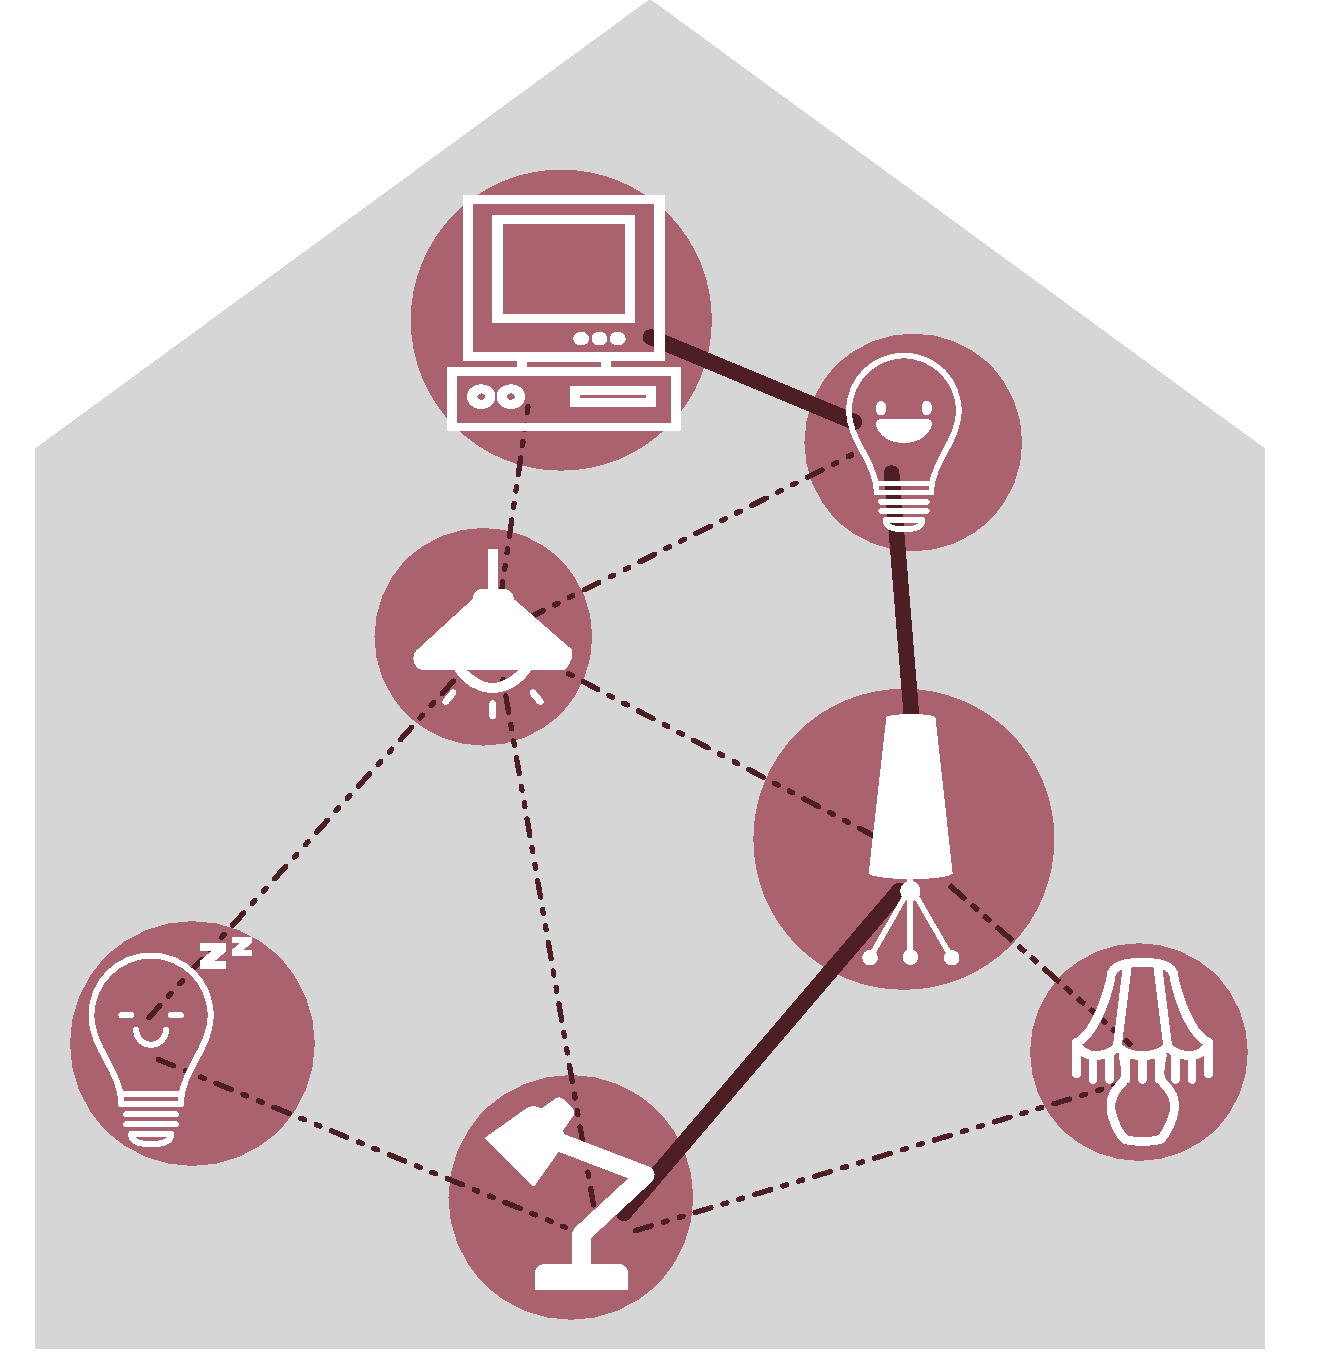
\includegraphics[width=\textwidth]{../images/route_centered_example}
                \caption{Example of a route-centered network: lights and control center in a smart home.}
                \label{fig:rc_img}
        \end{subfigure}%
        ~ %add desired spacing between images, e. g. ~, \quad, \qquad, \hfill etc.
          %(or a blank line to force the subfigure onto a new line)
        \begin{subfigure}[b]{0.5\textwidth}
                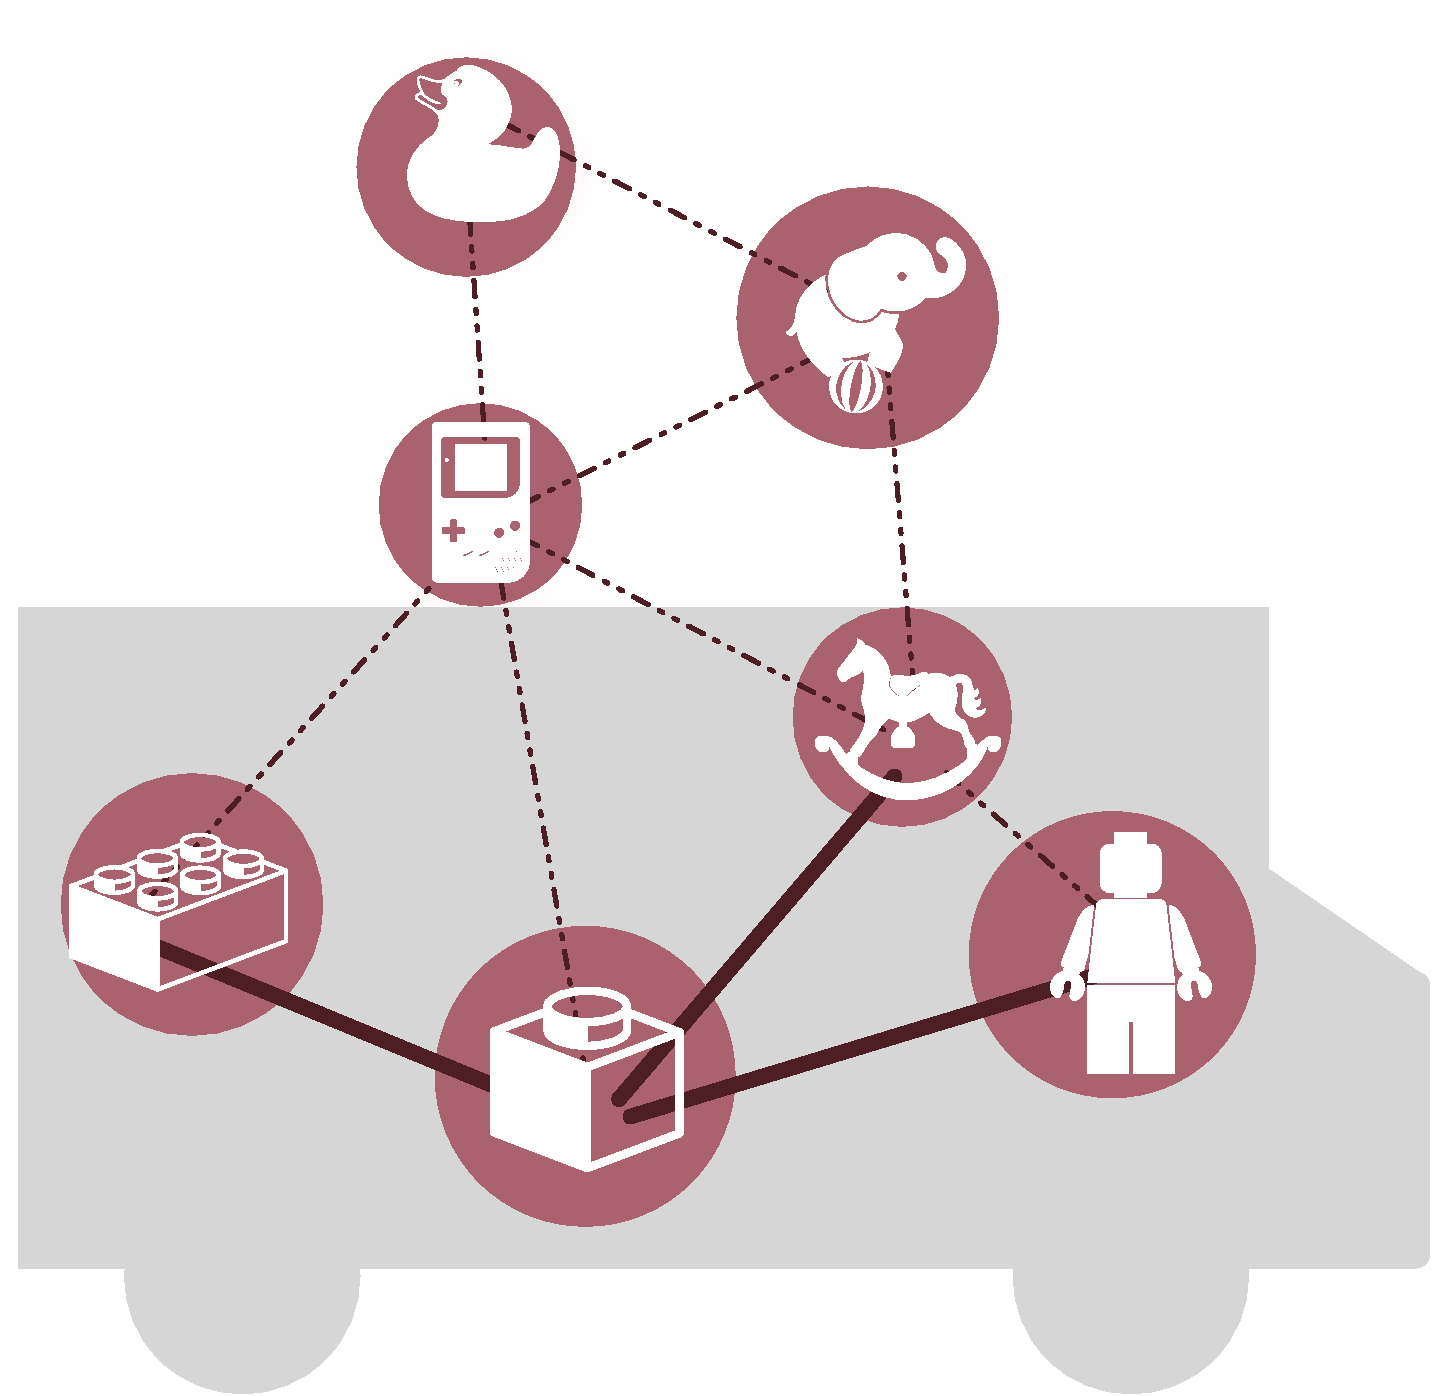
\includegraphics[width=\textwidth]{../images/area_centered_example}
                \caption{Example of an area-centered network: Goods in a delivery truck and warehouse}
                \label{fig:ac_img}
        \end{subfigure}
        \caption{Pictures of animals}\label{fig:animals}
\end{figure}

Hybrid protocols differ in the way they prioritize routes and decide which of them should be maintained proactively or set up reactively. There are two approaches to this, which this paper dubs the \emph{route-centered} and the \emph{area-centered} approach repectively.\\

The \emph{route-centered} approach serves networks in which some nodes, near or far, are more important than others. This is illustrated by fig. \ref{TODO}, which shows the different lamps of a house and the house's control center. Each lamp needs a stable connection to this control center, be it to switch on/off occaionally to confuse burglars, or exchange status info and configurations. Thus, this connection is maintained proactively, as indicated in the diagram by the thick straight line. Additionally, they may want to communicate with each other upon user interaction. Because this happens spontaneously and sparsely, the connections amongst all lamps are set up reactively, as indicated by the dotted lines.\\
Protocols with an \emph{area-centered} approach assume all nodes are equal in principle, but nearby nodes are more important than nodes which are farther away. 


\subsection{Architecture}
\label{subsec:architecture}
%==============================================================================

\section{Suitability for the IoT}
\label{sec:suitability}
%==============================================================================

\section{Conclusion}
\label{sec:conclusion}
%==============================================================================
tanslate old shit. Framework good, protocol bad. scope depends on deployment. framework may be able to accomodate that too. simulations mostly suck. real-world experiences are rare. hooray for testbeds!

\section{Outlook}
\label{sec:outlook}
%==============================================================================
figure out ways to slim down frameworks.
get real-world experiences. verify vermutungen oder auch nicht. so much to do!

\printglossaries

{\small
\bibliographystyle{ieeetr}
\bibliography{ausarbeitung}
}


\end{document}